\subsection{{\tt eaaCanal} package}\label{wseaacanal}

The management of an EAA canal requires a balancing of the flood
control and water supply requirements from adjacent water control
units while making optimal use of reservoirs and stormwater treatment
areas.  The \emph{pull} of water supply needs from directly connected
service/stormwater treatment areas and downstream outlets must
balanced with the \emph{push} of flood control releases from directly
connected service/stormwater treatment areas and upstream inlets.  The
{\tt eaaCanal} packages simulate the management of canal operations by
considering water supply and flood control needs separately.  The
water supply needs of the EAA canal are assessed by the {\tt eaaCanal}
water supply assessor (``wsAssessor'') package.  The wsAssesor
estimates the available water from directly connected sources (e.g.,
runoff from service areas and reservoirs) and quantifies the unmet
water supply requirements to be met by the regional system through
inlet water supply deliveries.  The flood control needs of the EAA
canal are assessed by the flood control assessor (``fcAssessor'')
package (see Section \ref{fceaacanal}).  The fcAssessor negotiates a
resolution between water supply and flood control differences at the
EAA canal outlets.

\begin{figure}[!htb]
 \begin{center}
  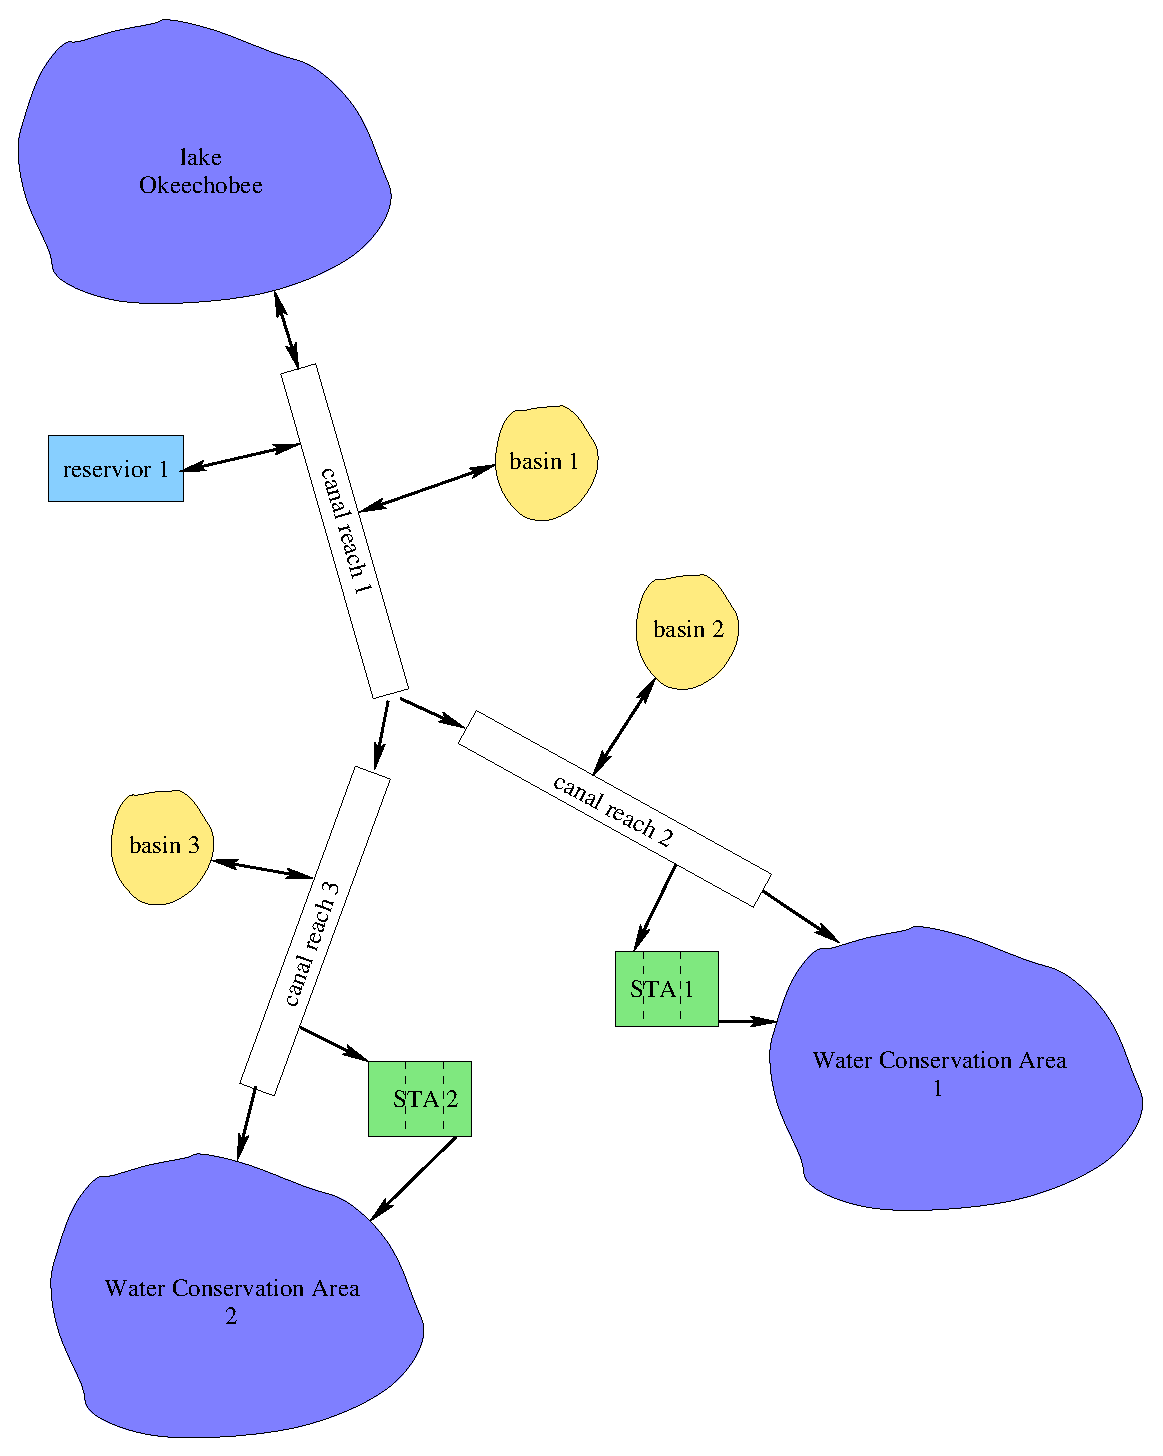
\includegraphics[scale=.5]{Graphics/eaacanal}
  \caption{\label{fig:eaacanal} EAA canal configuration}
 \end{center}
\end{figure}

The {\tt eaaCanal} assessor package is applied to each of the canal
reaches that connect an optional upstream reservoir (e.g., Lake
Okeechobee) to a downstream canal or storage area
(Figure \ref{fig:eaacanal}).  The {\tt eaaCanal} wsAssessor is
multipurpose, supervising the routing of water for:

\begin{enumerate}

 \item Flood control relief for an upstream EAA canal or reservoir;

 \item Water supply deliveries and flood control relief for adjacent
   agricultural service areas;

 \item Water supply deliveries and flood control relief for adjacent
   stormwater treatment areas;

 \item Runoff diversions to adjacent stormwater treatment areas for
   treatment;

 \item Runoff diversions to adjacent reservoirs for storage;

 \item Water supply deliveries from adjacent reservoirs; and

 \item Water supply deliveries to meet water supply needs in a
 downstream EAA canal or storage area;

\end{enumerate}

The water supply needs for the EAA canal are assessed by quantifying
the water supply requirements from adjacent service / stormwater
treatment areas and downstream outlets.  Water supply requirements are
met first by routing excess in the canal, e.g., runoff from adjacent
adjacent service / stormwater treatment areas, seepage and boundary
conditions.  Remaining water supply requirements are met by water
supply deliveries from directly connected and upstream reservoirs.

A flowchart schematic representation of the eaaCanal water supply {\tt
Assess()} function is shown in Figure \ref{fig:eaaCanalWS}.  The {\tt
eaaCanal} package for water supply has three primary operations:

 \begin{enumerate}

  \item Quantify water supply requirements from the adjacent service
  areas (SA's) and stormwater treatment areas (STA's);

  \item Quantify water supply requirements from the tailNode outlets;
  and

  \item Route local excess and compute the remaining deficit to be met
  by water supply deliveries from upstream reservoirs.

\end{enumerate}


\begin{figure}[!htb]
 \begin{center}
  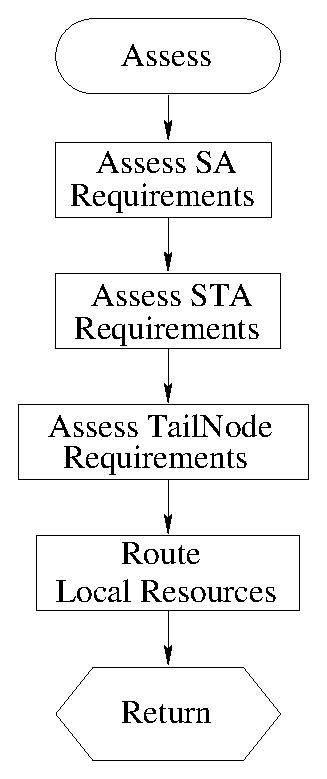
\includegraphics[scale=.5]{Graphics/eaaCanalWS}
  \caption{\label{fig:eaaCanalWS} EAA canal water supply Assess() function}
 \end{center}
\end{figure}

{\bf Compute Service / Stormwater Treatment Area Requirements}. The
water supply requirements for SA's and STA's are computed by executing
their respective water supply assessor (``wsAssessor'') functions.
Full implementation of the prioritization and allocation capabilities
in the {\tt eaaCanal} package requires a seamless integration with SA
and STA wsAssessors.  Currently, the {\tt eaaCanal} package requires
that the SA and STA wsAssessors use the {\tt std} package.  The {\tt
std} wsAssessor assesses water supply needs for the SA and STA by
computing their respective water supply requirements and distributing
the unmet water supply requirements to their water supply inlets.  The
{\tt std} package provides an option to designate the water supply
requirement with a landscape type.  For example, an agricultural WCU
would be given an ``ag'' designation.  Likewise, an environmental and
urban WCU's would be given ``env'' and ``urb'' designations,
respectively.  The {\tt eaaCanal} package uses these designations to
prioritize water supply deliveries and impose management constraints
based on landscape designation.

{\bf Compute TailNode Requirement}. A tailNode is defined as an outlet
connected to another EAA canal or a downstream storage area, such as a
Water Conservation Area.  A flowchart schematic representation for
computing the tailNode water supply requirement is shown in
Figure \ref{fig:eaaCanalWSTailNodes}.  The water supply assessor for
the downstream EAA canal is executed to quantify the water supply
requirement assigned to the tailNode.  Water supply requirement for a
downstream storage area is specified using a minimum flow constraint
for the tailNode.

\begin{figure}[!htb]
 \begin{center}
  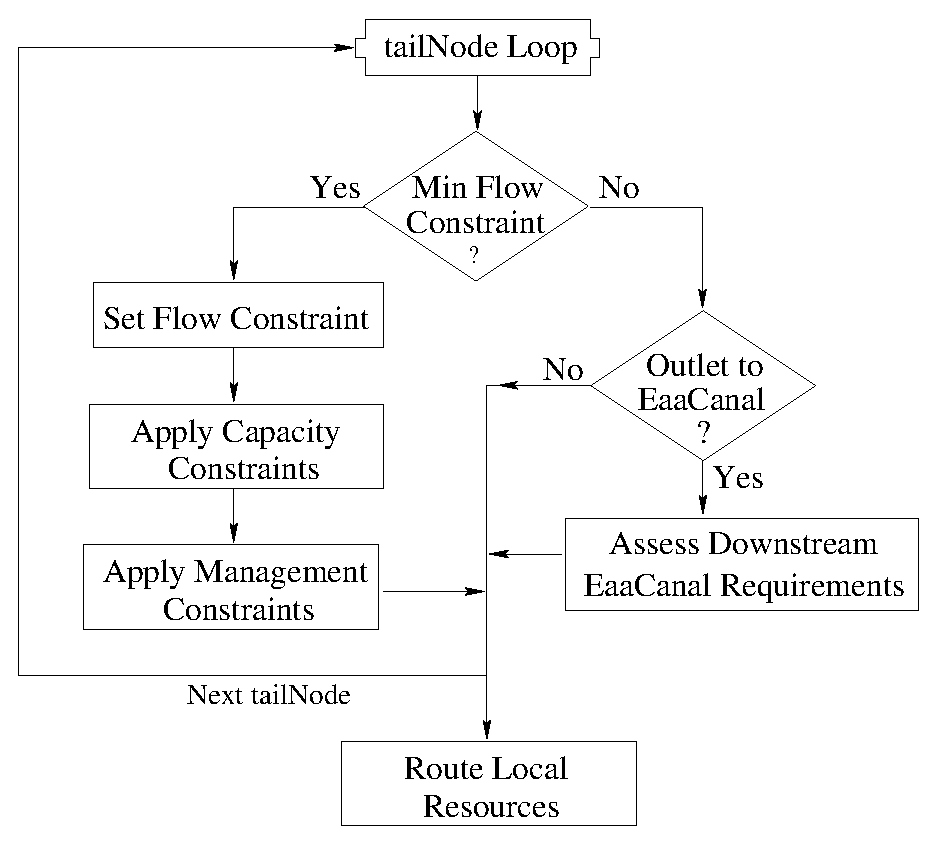
\includegraphics[scale=.5]{Graphics/eaaCanalWSTailNodes}
  \caption{\label{fig:eaaCanalWSTailNodes} EAA canal water supply tailNode assessment}
 \end{center}
\end{figure}

{\bf Route Local Resources}.  The {\tt eaaCanal} package uses the {\tt
RouteLocalResources()} function to quantify the portion of EAA canal
water supply requirement that can be met using local resources, such
as basin runoff and locally connected reservoirs.  The remaining water
supply requirements are met by regional deliveries through the
headNodes.

A schematic flowchart for the {\tt RouteLocalResources()} function is
presented in Figure \ref {fig:eaaCanalWSRouteLocal}.  The local and
regional deliveries required to meet the EAA canal water supply
requirements are assessed by following procedure:

\begin{enumerate}

  \item {\bf Estimate canal excess}.  Canal excess is defined as the
  net inflow from boundary conditions, groundwater seepage
  watermovers and estimated runoff from upstream SA's and STA's.
  Maintenance demand is defined as the inflow required to offset a
  computed negative excess.  Runoff from SA and STA WCU's is
  estimated by executing their respective fcAssessors and summing the
  resulting flood control releases through outlets discharging into
  the EAA canal.  The user can optionally restrict the use of SA or
  STA runoff for water supply.

  \item {\bf Route canal excess}.  Canal excess is routed to meet the
  water supply requirements at the canal outlets.  The water supply
  requirements are quantified by landscape type at each canal outlet.
  Canal excess is routed in ``landscape'' order, where the highest
  priority landscape types are processed first and the canal outlets are
  prioritized by downstream function: (1) outlets to stormwater
  treatment areas; (2) outlets to service areas; and (3) tailNode
  outlets.  Multiple outlets with the same function are processed in
  the order dictated by the keyword suffix specification.

  \item {\bf Route reservoir supply}.  Available supply from reservoirs
  directly connected to the canal is routed to meet the remaining
  water supply requirements at the canal outlets.  Available supply is
  routed to the water supply outlets in the same manner as the canal
  excess (i.e., in ``landscape'' order).  Reservoir releases are
  subject to management constraints that can be used to constrain
  releases based on landscape type.  Reservoirs with a headNode
  connection are processed through headNode deliveries.

  \item {\bf Compute canal deficit}.  The deficit for the canal is the
  summation of the remaining water supply requirements at the outlets,
  summed by landscape type.

  \item {\bf Set water supply requirements at headNodes}.  Canal
  deficits are resolved through regional deliveries at the headNodes.
  Water supply deliveries at a headNode are constrained by the
  remaining capacity of the headNode watermover, design capacity, and
  management constraints.  Canal deficits are distributed to multiple
  headNodes by: (1) priority order, or (2) defined fraction.  The
  priority order method assigns water supply requirements to the
  highest priority headNode in landscape order until all the canal
  deficits have been satisfied.  The defined fraction method
  distributes the canal deficit to the headNodes based on a user
  defined set of weights.
  
\end{enumerate}

\begin{figure}[!htb]
 \begin{center}
  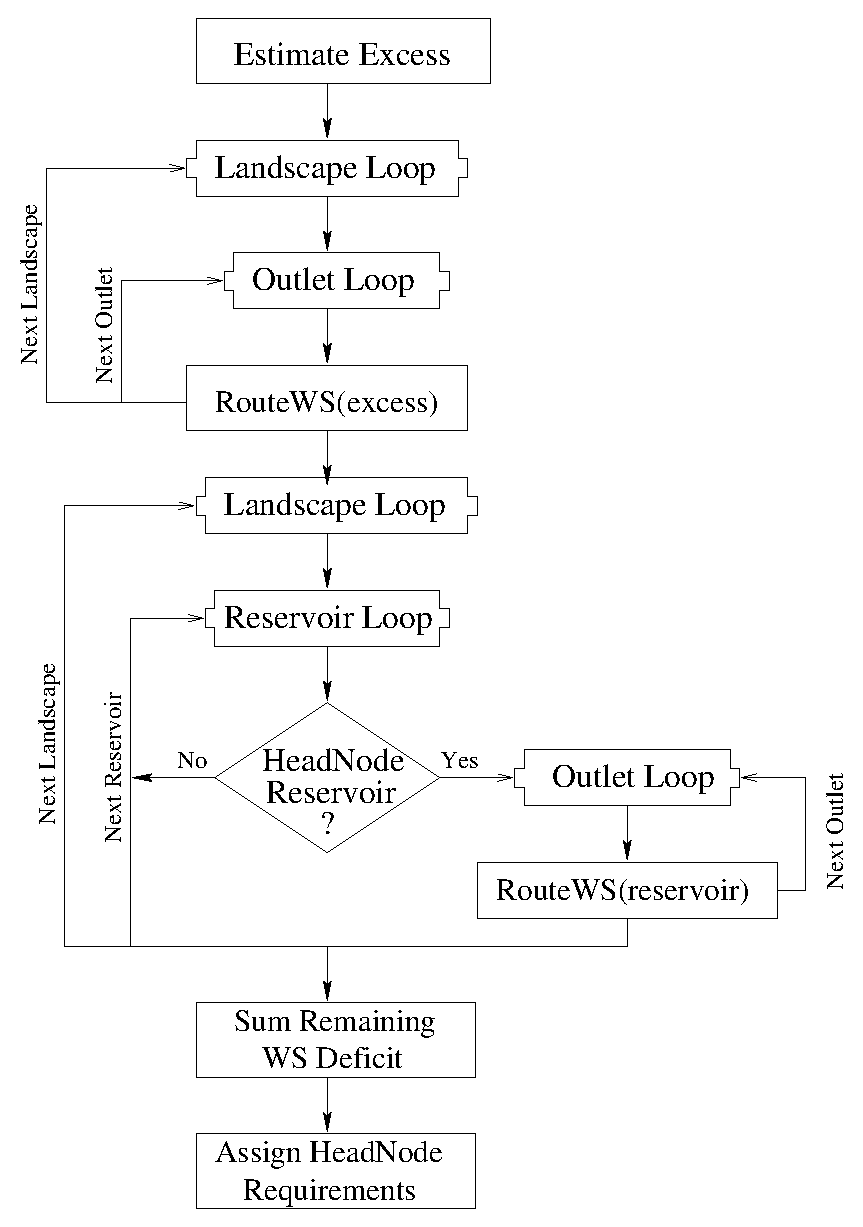
\includegraphics[scale=.5]{Graphics/eaaCanalWSRouteLocal}
  \caption{\label{fig:eaaCanalWSRouteLocal} EAA canal RouteLocalResources() schematic.}
 \end{center}
\end{figure}

The {\tt eaaCanal} prioritizes water supply releases based on the
destination's landscape type (see Table
\ref{table:eaacanalLandscape}):

\begin{table}[!htb]
 \begin{center}
  \footnotesize
  \caption{Prioritized landscape list for the {\tt eaaCanal} package. }\label{table:eaacanalLandscape}
  \begin{tabular}{p{1.0cm}p{2.0cm}p{10.0cm}}									\\[0.8ex]
   Priority	&Landscape 	&Description									\\
   \hline
   1		&maint		&inflow required to offset a computed negative excess in canal			\\
   2		&tribe		&water supply deliveries to tribal lands					\\
   2		&env		&environmental releases to maintain minimum water levels in an STA		\\
   3		&ag		&agricultural SA water supply delivery						\\
   4		&urb		&urban water supply delivery							\\
   5		&envTarg	&releases to meet target flows or water levels in environmentally sensitive areas \\
   6		&ws		&undesignated water supply delivery						\\
   \hline
  \end{tabular}
 \end{center}
\end{table}

